\clearpage

\thispagestyle{empty}

\chapter[Constant Communities in Networks]{Constant Communities in Networks} In this chapter we
address our first objective -- studying the dependence of community detection algorithms on the vertex ordering that leads to the
variability in the final output obtained.

\section{Introduction}

A fundamental problem in understanding the behavior of complex networks is the ability to correctly detect
communities. Mathematically, this
question can be translated to a combinatorial
optimization problem with the goal of optimizing a given metric of interrelation, such as modularity or
conductance. The goodness of community detection algorithms (see~\cite{lf2009} for a review) is often
objectively measured according to how well they achieve the optimization.

However, these algorithms can be applied to any network, regardless of whether it possesses a community
structure or not. Furthermore when the optimization problem is NP-hard, as in the case of
modularity~\cite{ng2002}, the order in which the vertices are processed as well as the heuristics can change
the results. These inherent fluctuations of the results associated with modularity have long been a source of concern
among researchers. Indeed the goodness of modularity as an indicator of community structure has also been
questioned, and there exist examples~\cite{gmc2010} which demonstrate that high modularity does not always
indicate the correct community structure. 
% Consequently, orthogonal metrics, such as conductance~\cite{lldm2008}
% (which is also NP-complete~\cite{brandes2008}) have been proposed.

Research in addressing the fluctuations in the results due to modularity maximization heuristics include identifying
stability among communities from the consensus networks built from the successive iterations of a non-deterministic
community detection algorithm (such as by Seifi et al.~\cite{sjri2012}). Lancichinetti et al.~\cite{lf2012}
proposed {\em consensus clustering} by reweighting the edges based on how many times the pair of vertices were
allocated to the same community, for different identification methods.  Ovelgonne et
al.~\cite{ogy2012} pointed out an ensemble learning strategy for graph clustering. Gfeller et al.~\cite{gcr2012}
investigated the instabilities in the community structure of complex networks. Finally, several pre-processing
techniques~\cite{PhysRevE.72., reidy} have been developed to improve the quality of the solution. These methods form
an initial estimate of the community allocation over a small percentage of the vertices and then refine this
estimate over successive steps.



\section{Defining Constant Communities}
All combinatorial optimization algorithms focus on compiling the differences in the results to arrive at an acceptable solution, and despite
these advances a
crucial question about the variance of results remains unanswered -- what does the {\it invariance} of the result tell us about the network
structure? In this chapter, we focus on the invariance in community detection as obtained by modularity maximization. Our results, on a set
of
scale-free networks, show that while the vertex orderings produce very different set of communities, some groups of vertices are always
allocated to the same community for all different orderings. We define the group of vertices that remain invariant as {\it constant
community} and the vertices that are part of the constant communities as {\it constant vertices}. Figure \ref{fig_constant} shows a
schematic diagram of
constant communities. In this figure, two colors (red and green) indicate two communities of
the network formed in each iteration. Combined results of two algorithms produce two constant communities (rectangular and circular
vertices).
Remaining one vertex (hexagonal shaped) is not included since it switches its community between the two algorithms.
Note that not all vertices in the network belong to constant communities. This is a key difference of constant
communities with the consensus methods~\cite{lf2012} described earlier. Consensus methods attempt to find the best (most stable or most
similar) community among all available results and thus include all the vertices. Constant communities, on the other hand, focus on finding
subgraphs where the cohesive groups can be unambiguously identified. As discussed earlier, communities obtained by modularity maximization
may
include vertices that can move from one group to another depending on the heuristic or the vertex ordering. The vertex groups obtained using
constant communities are invariant under these algorithmic parameters and, thereby, provide a lower bound on the number of uniquely
identifiable communities in the network. Although trivially each vertex can be considered to be a
constant community by itself, our goal is to identify the largest number of vertices (i.e., at least three or more) that can be included in
an invariant group.

\begin{figure}[!t]
\centering
\includegraphics[scale=0.3]{./texfiles/Chapter_2/Fig/Figure-1(Chakraborty).pdf}
\caption{ Schematic illustration of the formation of constant communities. }\label{fig_constant}
\end{figure}

The presence of such invariant structures can be used to evaluate the accuracy of the communities obtained when other independent methods of
verifications are unavailable.
However in many networks, constant communities constitute only a small percentage of the total number of vertices. To understand how other
non-constant vertices are allocated to communities, we show that by using constant communities we can significantly reduce the variations in
results (see Section \ref{sec:improve}). Thus, building from the more accurate results reduces the variance over the larger network. 



\section{Experimental Setup}

\subsection{Datasets} We conduct our experiments on networks obtained from real-world data as well as on a set of synthetically
generated networks using the LFR model~\cite{lfr2009}. The set of real-world networks is obtained from the instances available at the
10th DIMACS
challenge website~\cite{dimacs}. The networks, which are undirected and unweighted, include -- Jazz (network of jazz musicians;
$|V|=198, |E|=2742$)~\cite{jazz}, Polbooks (network of books on USA
politics; $|V|=105, |E|=441$)~\cite{polbooks}, Chesapeake (Chesapeake bay mesohaline network; $|V|=39, |E|=340$)~\cite{chesapeake},
Dolphin (Dolphin social network; $|V|=62, |E|=159$)~\cite{dolphin}, Football (American college football; $|V|=115,
|E|=1226$)~\cite{football}, Celegans (Metabolic network of C. elegans; $|V|=453, |E|=2025$)~\cite{PhysRevE.72.}, Power (topology of the
Western
States Power Grid of the USA; $|V|=4941, |E|=6594$)~\cite{Watts-1998} and Email (e-mail
interchanges between members of the Univeristy Rovira i Virgili; $|V|=1133, |E|=5451$)~\cite{email} (note that $|V|$ refers to the number
of vertices and $|E|$ refers to the number of edges).

%  All these networks
% exhibit scale-free degree distribution (see Figure \ref{deg}).




Networks generated using the LFR model are associated with a mixing parameter $\mu$ that represents the ratio of the external connections
of a node to its total degree. We create LFR networks based on the following parameters~\cite{lf2012}: number of nodes = 500, average
degree = 20,
maximum
degree = 50, minimum community size = 10, maximum community size = 50, degree exponent for power law = 2, community size exponent = 3. We
vary the value of $\mu$ from 0.05 - 0.90. Low values of $\mu$ correspond to well-separated communities that are easy to detect and
consequently these networks contain larger percentage of constant communities. As $\mu$ increases, communities get more ambiguous and
community detection algorithms provide more varied results leading to fewer vertices being in significantly sized constant communities.

% \begin{figure}[t]
%  \centering
% \includegraphics[scale=0.3]{./texfiles/Chapter_2/Fig/cumulative_deg_dist.pdf}
% \caption{{\bf Cumulative degree distributions of the real-world networks.} The networks, regardless of the number of constant
% communities
% present, exhibit power-law degree distribution.}\label{deg}
% \end{figure}


\subsection{Community Detection Algorithms}
We select two popular agglomerative modularity maximization techniques -- the method proposed by Clauset et al.~\cite{cnm2004}
(henceforth referred to as the {\em CNM} method) and the method proposed by Blondel et al.~\cite{bgll2008} (henceforth referred to as
{\em Louvain}
method). Both these methods initially start by assigning one vertex per community. Then at each iterative step, two communities whose
combination most increases the value of modularity are joined. This process of joining community pairs is continued until the value of
modularity no longer increases. The Louvain method generally produces a higher value of modularity than CNM, because it allows vertices to
migrate across communities if that leads to a more optimum value.



\subsection{Degree Preserving Order}\label{order} 
Ideally, the total number of different orderings to be tested should be equal to the factorial of the
number
of vertices in the network. However, even for the smallest network in our set (Chesapeake with 39 vertices) this value is astronomical. We
therefore restrict our permutations to maintain a {\it degree-preserving} order. The vertices are ordered such that if degree of $v_i$ is
greater than the degree of $v_j$, then $v_i$ is processed prior to $v_j$.

In addition, to reducing the number of vertex permutation, degree-preserving permutation also has another important advantage. Recall
that
the networks in the test suite have few vertices with high degrees and a lot with low degrees. Therefore, arranging the high degree vertices
earlier pushes most of the fluctuations towards the later part of the agglomeration process. This ensures
that the sub-communities formed initially are relatively constant and only later do the divergence in community memberships take place.
Clearly, such orderings based on decreasing degrees are geared towards facilitating low variance in communities. If {\it this ordering}
does not produce constant structures, it makes a very strong case about the inherent fluctuations that underlie modularity
maximization methods.



\section{Identifying Constant Communities} In order to identify constant communities from a network, we permute the order of the vertices,
and then apply a
community detection algorithm to each of the permuted networks. The results vary across permutations. We select the groups of vertices that
are always allocated together across all the permutations and mark them as constant communities. The rationale behind this process is
that these vertices must have some intrinsic connectivity properties that force them to stay together under all orderings.


\begin{table}[!t]
 \centering
\caption{Comparison of the constant communities obtained from Louvain (LVN) with those obtained from CNM and Infomap (INFO) algorithms using
NMI.}\label{nmi_real}
\scalebox{0.7}{
\begin{tabular}{|c|c|c|c|c|c|c|c|c|c|}
\hline
\textbf{Networks}& & Jazz & Chesapeake & Dolphin & Football & Polbooks & Celegans & Email & Power \\\hline
\multirow{2}{*}{\textbf{NMI}}& LVN vs. CNM &  0.8856& 0.8429 & 0.8663 & 0.8765 & 0.8950 & 0.9232& 0.8103& 0.8097\\\cline{2-10}
&LVN vs. INFO &  0.8235& 0.7928 & 0.9722 & 0.8824 & 0.8239 & 0.9144 & 0.8072 & 0.7856\\\hline
\end{tabular}}
\end{table}

To implement the vertex permutation, we adopt a stochastic degree-preserving scheme as discussed in Section \ref{order} that can arrange the
vertices based on the descending
order of their degrees.  The ordering of the set of vertices with the same degree is permuted. By applying this method we preserve the
relative ordering of the degrees of the vertices since it is well-known that node-degrees constitute a fundamental network property. 
% We have
% also observed that the random
% permutations producing high modularity usually preserve a degree-descending order of vertices and the ones that result in low modularity
% usually are outcomes of cases where the algorithm would start executing from a low-degree vertex. 
Thus, our permutations prevent us from the
possibility of getting confined in a local maximum of the modularity.

In order to identify these
communities, for each network in the test suite, we apply CNM (and Louvain) method over different permutations of the vertices and
then
isolate the common groups that are preserved across the different orderings. These common groups of vertices are
marked as the constant communities for the respective
network.

We further observe based on the high ($>$ 0.80) Normalized Mutual
Information (NMI)  \cite{nmi} (see Section \ref{sec:ground-truth_metric}) values that the overlap
between the constant communities obtained from the two methods is considerable~\cite{nmi_2} (see Table \ref{nmi_real}). One might
argue that the constant communities are highly dependent on the underlying optimization functions (such as modularity) or the methods (such
as agglomerative method) used in the community detection algorithms. To cross-check this, we further detect the constant communities using
another very popular non-deterministic community
finding
algorithm called {\em Infomap} \cite{info} which is not an agglomerative
method but tries to minimize the minimum description length of the bit
sequence generated by a random walk. We observe a similar high overlap between the constant communities obtained from Louvain and
Infomap (see Table \ref{nmi_real}). Therefore, in the interest of space and
clarity we confine our discussion about the properties of constant communities to those obtained from the Louvain method.


\begin{figure}[!t]
\centering
\includegraphics[scale=0.2]{./texfiles/Chapter_2/Fig/Figure-2(chakraborty).pdf}
\caption{ Sensitivity of each network across 5000 permutations. X-axis is rescaled by a constant factor of 100 for better
visualization. }\label{fig:sensitivity}
\end{figure}



\section{Characteristics of Constant Communities}
In this section, we identify some interesting characteristic properties of constant communities observed in the real-world networks.


\subsection{Sensitivity of Community Structure to Vertex Perturbations} \label{sensitive}
In our first experiment, we study how the community structures of
the
networks change under vertex perturbations. Since constant communities are the groups
of vertices that remain invariant, we measure the change in community structure based on the number of constant
communities. We define \textit{sensitivity} ($\phi$) as the ratio of the number of constant communities to the
total number of vertices. If $\phi$ is 1 then each vertex by itself is a constant community (the trivial case),
thus there is no consensus over the set of communities obtained over different permutations. The higher
the sensitivity metric, the fewer the vertices in each constant community and, therefore, this metric is useful
for identifying networks that do not have a good community structure under modularity maximization. Note that this metric will be used
further in Section \ref{ordering} to quantify degeneracy of solutions of a community detection algorithm. 

The sensitivity of each network is given in Figure \ref{fig:sensitivity}. The x-axis indicates the number of
different permutations of the vertices and the y-axis plots the value of the sensitivity. We observe that for
most of the networks the number of constant communities become stable within the first 100 permutations, and the
sensitivity values are low. This indicates that there can potentially exist very strong groups in these networks
that have to be together to achieve high modularity. However, for networks such as Power and Email,
the number of constant communities keeps increasing until the values of $\phi$ are close to 1. Thus, the
community detection results for these two networks are extremely sensitive to the vertex perturbations. This
implies that the communities (if any) in these two networks are not tightly knit, i.e., very ``amorphous''.





\subsection{Percentage of Constant Communities} We further define
the
\textit{relative size} ($\xi$) of a constant community as the ratio of the number of vertices in that constant community to the total
number
of vertices in
the network and the \textit{strength} ($\Theta$) as the ratio of the edges internal to the constant community to the edges external (i.e.,
one end point of the edge is inside the constant community while the other is outside) to the
constant community. Figure \ref{intr_extr} plots the relative size (in percentage) of the constant communities with respect to their
strength. If the strength of a constant community is above 1 (above 0 in log scale) then the number of internal
edges in the community is larger than the number of external edges. The higher the value, the more tightly
connected is the community. We notice that the value of relative size ranges from 0-34, with a larger cluster of
values around 0-5. This shows that most of the constant communities contain very few vertices with respect to
the network size. If the relative size of the constant communities is low then the remaining vertices have more
freedom in migrating across communities, making the community structure weaker. We observe that, despite there
being more constant communities of low relative size, there are some networks that have multiple constant
communities with relative size over 15\% of the total number of nodes indicating that they have a much stronger
community structure. These include Jazz, followed by Dolphin and then Polbooks and Chesapeake.

\begin{figure}[!t]
\centering
\includegraphics[scale=0.22]{./texfiles/Chapter_2/Fig/Figure-3(chakraborty).pdf}
\caption{ Comparison between the relative size and strength of the constant communities. X-axis plots the
relative size in percentage, and Y-axis (in logarithmic scale) plots the strength. The plot is vertically divided at x = 17 that could help
systematically analyze the distribution of the points.
}\label{intr_extr}
\end{figure}

Relative size and strength together provide an estimate of which networks have good community structure. If we divide the x-axis at
roughly the
mid-point of the range and the y-axis at 1, then we obtain four quadrants each representing different types of community structures.
The first quadrant (upper right)
contains communities that have high relative size as well as high strength. Networks containing a large number of such constant
communities
are less likely to be affected by perturbations. Diagonally opposite is the third quadrant (lower left), which contains communities of low
relative size and low strength. As discussed earlier, networks having communities predominantly from this quadrant will produce
significantly
different results under perturbations and are likely to not have a strong community structure under modularity maximization. The second
quadrant (upper left) contains the
groups of vertices that are strongly connected but have small relative size. This indicates that there are some pockets of the network
with
strong community
structure. The fourth quadrant (lower
right) represents communities with high relative size but low strength. In this set of experiments it is empty, and we believe that
this area will be sparsely populated, if at all. This is because networks having such communities will have a very special structure:
strongly connected groups of very few vertices with many spokes radiating out to account for the high number of external communities.



\subsection{Pull from External Connections}\label{sec:rel_perm}
We note in Figure \ref{intr_extr} that there are several constant communities whose strength is below one,
i.e., they have more external than internal connections. This is counterintuitive to the idea that a strong community should have more
internal connections. Indeed, modularity maximization methods always tend to create communities whose strengths are greater than
one. However, the structure of some of the constant communities belies this convention.

We observe that in these cases, the external connections are distributed across different communities. Furthermore, the number of
connections to
any one external community is always lower than the internal connections. Based on this observation, we hypothesize that a group of
vertices are likely to be placed together so long as the internal connection is greater than the connections to any one single external
community. In such a scenario, the vertices within the community do not experience a significant ``pull'' from any of the external
communities that  can
cause them to migrate, and therefore, their propensity to remain within their own communities is high. We quantify this observation as
follows:


\begin{figure}[!t]
\begin{minipage}[b]{0.4\linewidth}
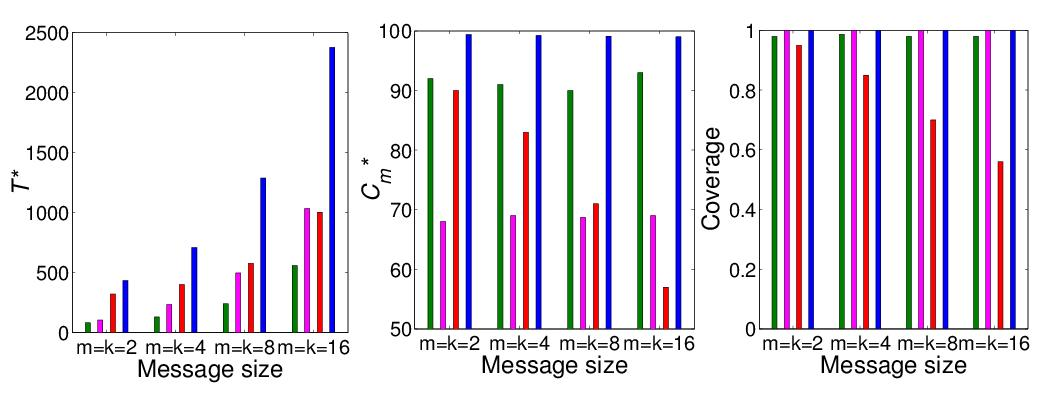
\includegraphics[width=2.8 in]{./texfiles/Chapter_2/Fig/fig2.jpg}
\end{minipage}
\hfill
\begin{minipage}[b]{0.45\linewidth}
 \includegraphics[width=2.4 in]{./texfiles/Chapter_2/Fig/fig1.jpg}
\end{minipage}
\caption{(Left) Schematic diagram illustrating the computation of the relative permanence of the vertices; (Right) distribution of
relative permanence values.}\label{pull}
\end{figure}

% \begin{figure}[!t]
% \centering
% \includegraphics[scale=0.2]{./texfiles/Chapter_2/Fig/Figure-4(chakraborty).pdf}
% \caption{{\bf Top: Schematic diagram illustrating the computation of the relative permanence of the vertices. Bottom: Distribution of
% relative permanence values.} X-axis plots the value of $\Omega$ and y-axis plots the cumulative fraction of vertices $P(\Omega)$
% exhibiting
% that $\Omega$. Both axes are in logarithmic scale.}\label{pull}
% \end{figure}


Let $v$ be a vertex in a constant community; further, let $D(v)$ denote the degree of $v$, and $EN(v)$ and
$IN(v)$ denote the number of external and internal neighbors of $v$ respectively (i.e., $D(v)=IN(v)+EN(v)$). We
also assume that the $EN(v)$ external neighbors are divided into $k$ external groups, and $ENG(v)$ denote a set
of $k$ elements where the \textit{i}th element in the set represents the number of neighbors of $v$ belonging to
the $i^{th}$ external group. For instance, consider the vertex $A$ in $CC_1$ in Figure \ref{pull} (left),
$D(A)=9, IN(A)=3, EN(A)=6$ and $ENG(A)=\{3,2,1\}$ (i.e., three external neighbors in $CC_2$, one external
neighbor in $CC_3$, and two external neighbors in $CC_4$). Similarly, we calculate $ENG(v)$ for each vertex in
the network and form a list $DENG(G)$ by taking union over all $ENG(v)$, that is, only  unique entries across
$ENG(v)$ get listed in $DENG(G)$ (see Figure \ref{pull} (left)). The list is then ranked in ascending order, i.e., the group
with lowest number of external neighbors is ranked 1, the group with second lowest external neighbors is ranked 2 and so on.
The intuition behind this ranking is that we are more interested in how distinct the external neighbor groups are, rather than the
absolute size of the external neighbor groups. Moreover, by ranking, we can reduce the skewness of the range of external group size. This
rank would therefore signify the intensity of the pull of the particular external community and its inverse signifies the degree
of stability of the vertex $v$. 

% This formulation is motivated by the standard statistical measure called Mean Reciprocal Rank
% (MRR)~\cite{mrr} which is the average of
% the reciprocal ranks of results for a sample of queries.


For a particular vertex, if the inverse rank of each of the external group is equal to one, it would point to the fact
that all its external neighbors are diversely distributed (i.e., well-spread), and therefore the pull
experienced should be minimum; in contrast, if the value is much lower than one, it would imply that the  vertex
experiences a strong pull from its external neighbors. We define the {\it strength} of a vertex {\it v},
$\theta(v)$, as the ratio of the internal neighbor ($IN(v)$) to the external neighbor ($EN(v)$) of vertex $v$
similar to  the strength ($\Theta$) of a constant community defined earlier. Mathematically, the suitably
normalized value of $relative\ permanence$, $\Omega(v)$, of a vertex $v$ in a constant community can be expressed as:


\begin{equation}
\Omega(v)= \theta(v) \times \frac{\sum_{i=1}^k {\frac{1}{Rank(ENG_i(v))}}}{D(v)}
\end{equation}

where $Rank(ENG_i(v))$ denote the rank (retrieved from the {\it DENG(v)} list) of the $i^{th}$ element in $ENG(v)$. This metric
indicates the propensity of a vertex to remain in the same community regardless of any algorithmic parameters. 

%{\bf Note that, if a vertex
%has no external connection, its relative permanence is considered as one since in that case, it is the most stable vertex in the network.
%The two extremal cases of $\Omega(v)$ are: (i) the external neighbors are uniquely distributed into different communities and
%(ii) all the external neighbors are within one single community. For the first case, $\sum_{i=1}^k {\frac{1}{Rank(ENG_i(v))}}=EN(v)$
%and
%$\Omega(v)=In(v)/D(v)$. For the second case, $k=1$ and $Rank(ENG_1(v)) \leq EN(v)$. Therefore, $\Omega(v) \leq [\frac{IN(v)}{D(v)} \times
%\frac{1}{EN(v)^2}]$}.

Figure \ref{pull} (left) presents a schematic diagram for computing relative permanence of vertices within the communities. Figure
\ref{pull}
(right)
plots the
cumulative
distribution of the relative permanence over the vertices in all networks. The x-axis indicates the value of the relative permanence and
the
y-axis, the cumulative fraction of vertices having the corresponding relative permanence value.
The nature of the cumulative permanence distribution of the vertices is roughly same for all networks except Email and Power. The
distinguishing nature of the curves for Email and Power graphs compared to the other graphs indicates that very few number of vertices in
these two networks have higher relative permanence values and therefore experience more ``pull'' from the external communities.
 Another observation is that a high fraction of
vertices in Jazz, Polbooks, Dolphin and Celegans have
relative permanence close to one. These vertices are more ``stable'' compared to the other vertices in the respective networks.


 



\begin{center}
\begin{algorithm}[!ht]
 
\tiny
   
%\fbox{\begin{minipage}[t]{0.8\columnwidth} 
\caption{Modularity maximization using constant communities}  

%{\bf Algorithm 1: Modularity Maximization Using Constant Communities}
%\noindent\makebox[\columnwidth]{\rule{\columnwidth}{0.4pt}}
  {\bf Input:}  A network (graph) $G=(V,E)$; Community detection algorithm $A$.\\
  {\bf Output:} Set of constant communities ${CC_1}$, \ldots${CC_k}$; Modularity $Q$

\begin{algorithmic}[]
  
  \Procedure{Finding Constant Communities}{}
  \State{Sort vertices in $V$ in degree descending order}
  \State {Apply degree preserving permutation $P$ to vertices such that degree($v_i$) $\ge$ degree($v_{i+1}$) in $P$.}
  \State {$|P|$ is number of degree preserving permutations applied.}
  \State{ Initialize  array $Vertex[|V|][|P|]$ to -1}  \hfill \Comment{$Vertex[|V|][|P|]$ will store the community membership of
the vertices in each permutation}
 
  \State{Set $i=0$} \hfill \Comment{This variable indicates the permutation index}
  
   \ForAll {$P_i \in P$} \hfill  \Comment{Detect community memberships of the vertices in each  permutation using $A$ and
store them
in
$Vertex$}
    \State {Apply algorithm $A$ to find the communities of the permuted network $G_{P_{i}}$}
    \If {Vertex $v$ is in community $c$} 
       \State {$Vertex[v][i]=c$} \hfill \Comment{Vertex $v$ in permutation $P_i$ belongs to community c after applying $A$
to
$P_i$}
    \EndIf 
      \State {$i=i+1$}
    \EndFor
    
    \State{Set $j=0$}  \Comment{This variable indicates the index of the constant community}
    \ForAll{ $v \in V$} \Comment{Detecting constant communities using the community  information stored in $Vertex$}
	\If {vertex $v$ is not in a constant community}
	  \State {Create constant community $CC_j$}
	  \State {Insert $v$ to $CC_j$}        \hfill         \Comment{All $CC_{j}s'$ are the constant communities}
	    
        \ForAll{ $u \in V \setminus CC_j$}
        
        \If{ $Vertex[v][i] = Vertex[u][i]$, $\forall$ $i=1$ to $|P|$} \hfill \Comment {Check for the exact matching of
community
memberships of
{\it u} and {\it v}}
        \State {Insert $u$ to $CC_j$ }
        \EndIf
        \EndFor
    
      \EndIf
    \State {$j=j+1$}
    \EndFor


\EndProcedure

  \Procedure{Computing Modularity}{} 
  
\State{ Set of constant communities in $CC$}
\ForAll { $CC_j \in CC$}   \Comment{Create intermediate small, weighted network}
  \State {Combine vertices in $CC_j$ into a super-vertex $X_j$}
  \State {Replace edges from $X_j$ to another vertex $X_i$ by their aggregate weight} \hfill \Comment{For the self-loop, $i=j$} 
\EndFor
\State {Sort vertices of collapsed network, $G'$, in degree descending order}
\State {Apply community detection method $A$}
\State {Unfold all $X_j$ in $G'$ and compute the modularity $Q$}
\EndProcedure

\end{algorithmic}
%\end{minipage}}}
\end{algorithm}
\end{center}


\section{Constant Communities for Improving Modularity}\label{sec:improve}
 We note that in many networks (such as Football and Celegans) constant communities form only a small percentage of the vertices. Thus,
finding only the constant communities may not provide adequate information about the relationship amongst the rest of the vertices. We
therefore leverage on the invariant results in the first and second quadrants of 
Figure \ref{intr_extr} as building blocks to identify larger communities.






\begin{table}
\caption{Modularity before and after pre-processing for real networks (left) and for different values of mixing parameter ($\mu$) over LFR
graphs (right)}\label{modularity}
\parbox{.49\linewidth}{
\centering
\scalebox{0.6}{
\begin{tabular}{|c|c|c|c|c|}
 \hline
 & \multicolumn{4}{|c|}{Louvain}\\
\cline{2-5}
Networks & \multicolumn{2}{|c|}{Before pre-processing} & \multicolumn{2}{|c|}{After pre-processing} \\
\cline{2-5}
&  Mean ($m_q$) & Var ($\sigma_q$) & Mean ($m_q$) & Var ($\sigma_q$) \\
\hline
Jazz &  0.448 & 3.13e-6 & 0.452 & 0 \\
\hline
Chesapeake &  0.301 & 1.17e-5 & 0.303 & 3.36e-33 \\
\hline
Polbooks &  0.539 & 1.74e-5 & 0.557 & 1.24e-32 \\
\hline
Dolphin & 0.543 & 1.76e-5 & 0.550 & 0 \\
\hline
Football &  0.610 & 2.01e-5 & 0.623 & 0 \\
\hline
Celegans & 0.438 & 2.89e-5 & 0.442 & 1.33e-26 \\
\hline
Email & 0.542 & 6.89e-5 & 0.568 & 0.95e-12 \\
\hline
Power & 0.936 & 1.09e-5 & 0.937 & 2.25e-10 \\
\hline
\end{tabular}}
}
\hfill
\parbox{.49\linewidth}{
\centering
\scalebox{0.65}{
\begin{tabular}{|c|c|c|c|c|c|}
  \hline
 & &\multicolumn{4}{|c|}{Louvain} \\
\cline{3-6}
$\mu$& Planted&\multicolumn{2}{|c|}{Before } & \multicolumn{2}{|c|}{After}\\
 & Modularity& \multicolumn{2}{|c|}{pre-processing} & \multicolumn{2}{|c|}{pre-processing} \\
\cline{3-6}
&  &Mean($m_q$) & Var($\sigma_q$) & Mean($m_q$) & Var($\sigma_q$) \\
\hline
0.05 & 0.878 & 0.834 & 1.98e-24 & 0.877 & 0 \\
\hline
0.10 & 0.817 & 0.802& 2.28e-28& 0.817& 0\\
\hline
0.20 & 0.716 & 0.690& 5.74e-7& 0.686& 0\\
\hline
0.50 & 0.440 & 0.385& 2.05e-6 & 0.389& 1.58e-28\\
\hline
0.70 & 0.223 & 0.298& 9.70e-10& 0.219& 1.04e-28\\
\hline
0.90 & 0.029 & 0.225& 4.25e-10& 0.205& 5.64e-28\\
\hline
\end{tabular}}
}
\end{table}



We first permute the vertices 5000 times in degree-descending order i.e., each of the permutations preserves the constraint
that if vertex
$v_i$ is placed before $v_j$ in the sequence then $degree(v_i) \ge degree(v_j)$. Then for each of these permutations,
we run Louvain algorithm and obtain the community structure (and the modularity value). Table~\ref{modularity} (left) shows the
mean modularity (and its variance) obtained by averaging the modularity values of all iterations. Next, from these community structures
obtained across the different permutations, we
detect the constant
communities and combine them into super-vertices.
This process creates a smaller network as well as ensures
 that the vertices in the constant communities always stay together. Then we execute a modularity maximization algorithm
over the entire network. We compute the variance in results by executing
the
underlying modularity maximization algorithm individually over 5000 permutations, in each case maintaining the degree-preserving order
(see Algorithm 1). As
shown in Table~\ref{modularity}
(left), combining constant communities as a pre-processing step both increases the mean modularity value as well as reduces the variability
across permutations for real-world networks.

We also observe that the variance becomes 0 or very low for the networks which have significant number of constant
communities in the first and second quadrants of Figure \ref{intr_extr}. The results obtained from the other
networks with high sensitivity, such as Email and Power, still indicate some variance although the value is less pronounced.


 These observations on real-world networks lead us to believe that pre-processing using constant communities is more effective if a network
has strong community structure. To test this hypothesis, we create
LFR graphs with mixing parameters from 0.05 to 0.90. Low mixing parameters indicate strong community structure. For the LFR
graphs, we repeat the same set of experiments as discussed above and obtain the mean modularity and its variance. As shown in
Table~\ref{modularity} (right), pre-processing using constant communities also helps increase the modularity value and reduces variability
of the results in the LFR graphs.

Another advantage of LFR networks is that we know the ``ground-truth'', i.e., the correct distribution of
communities (exact number of vertices in each community and the number of in-community connections between them). We use
NMI to
compare the obtained communities, with and without using the pre-processing step with the ground-truth community structures of LFR
graphs
for different mixing parameters. As
shown in Figure \ref{nmi}, when the community structure is strong (low mixing parameter), using constant
communities pushes the result towards the ground-truth. In contrast, when the
community structure is not well-defined (high mixing parameter), use of constant communities does not mimic the
community distribution of the ground-truth, because there can be many variations of community distribution in
such networks that lead to high modularity. These results once again highlight the significance of constant
communities.

\begin{figure}[!t]
\centering
\includegraphics[scale=0.25]{./texfiles/Chapter_2/Fig/Figure-6(chakraborty).pdf}
\caption{Variation of NMI for different values of mixing parameters. The broken line corresponds to the experiment without the
pre-processing step
and the solid line to the experiment after using the pre-processing step.}\label{nmi}
\end{figure}



\section{Relative Ranking of Constant Communities} A constant community is meaningful if it is large in size (high $\xi$)
or it
has high relative permanence ($\Omega$). We calculate the relative permanence of a constant community by averaging the relative
permanence of its constituent vertices. We experiment to see  which one of these two properties is more important in determining
high modularity. To do so,
we order the constant communities according to (a) decreasing order of $\xi$ and (b) decreasing order of $\Omega$. We combine the
constant communities into super-vertices one by one following the order obtained from (a) and (b) separately. After each combination, we
compute the modularity and compare the value with the average modularity (over 5000 permutations) obtained by using the Louvain
method without any pre-processing. 

Figure \ref{big} compares the modularity obtained by collapsing constant communities according to the order obtained from (a) (dotted blue
line) and (b) (dotted green lines). For almost all the networks, there is a transition where the modularity values cross over the mean
modularity (solid red line). Once this transition takes place, the modularity
values generally remain above (or at least equal to) the mean modularity.  This critical point indicates the smallest fraction of constant
communities required to outperform the original algorithms. We observe further that
the green lines (ordered according to $\Omega(v)$) generally reach the critical point earlier than the blue lines (ordered according to
 $\xi$), indicating that $\Omega(v)$ is a better indicator of constant communities. 



\begin{figure}[t]
\centering
\includegraphics[scale=0.25] {./texfiles/Chapter_2/Fig/Figure-7(chakraborty).pdf}
\caption{ Modularity after partially collapsing the constant communities.  The broken blue lines are in decreasing order
of size and the broken green lines are in decreasing order of relative permanence. The red lines depict the mean modularities
without using constant communities.}\label{big}
\end{figure}



\section{Case Study} The significance of constant community in a network can be further understood if we consider networks where
nodes have specific functionalities associated with them. We hypothesize
that
in such a network a constant community would represent indispensable functional blocks that reflect the defining characteristics of the
network. In order to corroborate this hypothesis we conduct a case study on a specific type of linguistic network constructed from the
speech sound inventories of the world's languages~\cite{pho}. The sound inventory of a language comprises a set of consonants and vowels
also
sometimes together known as {\em phonemes}. In order to unfurl the co-occurrence principles of consonant inventories, Mukherjee
et al.~\cite{pho}
constructed a network (phoneme-phoneme network or PhoNet) where each node is a consonant and an edge between two nodes denotes if the
corresponding consonants have co-occurred in a language. The number of languages in which the two nodes (read consonants) co-occur defines
the
weight of the edge between these nodes. Note that each node here has a functional representation since it can be represented by means of
a set of phonetic features (e.g., bilabial, dental, nasal, plosive etc.) that indicate how it is articulated. Since this is a weighted
graph, we suitably define a threshold to construct the unweighted version. We detect constant communities of PhoNet and observe that each
such graph (see Table~\ref{phon}) represents a {\em natural class}, i.e., a set of consonants that have a large overlap of the
features~\cite{pho}. Such groups are frequently found to appear together across languages, and linguists describe this observation through
the principle of {\em feature economy}~\cite{pho}. According to this principle, the speakers of a language tend to be economic in choosing
the features in order to reduce their learning effort. For instance, if they have learnt to use a set of features by virtue of learning a
set of sounds, they would tend to admit those other sounds in their language that are combinatorial variations of the features already
learnt -- if a language has the phonemes /p/ (voiceless, bilabial, plosive), /b/ (voiced, bilabial, plosive) and /t/
(voiceless, dental, plosive) in its inventory then the chances that it will have /d/ (voiced, dental, plosive) is disproportionately
higher compared to any other arbitrary phoneme since by virtue of learning to articulate /p/, /b/ and /t/ the speakers need to learn no new
feature to articulate /d/. Identification of constant communities therefore systematically unfolds the natural classes
and provides a formal definition for the same (otherwise absent in the literature). 
%We plot in Figure \ref{phonet} the average hamming distance between the feature vectors of phonemes forming a constant
% community versus the community size. The average hamming distance is significantly lower in the case when a set of randomly
% chosen phonemes are
% grouped together and assumed to represent a community with varying sizes as that of the constant communities. 
Further, we observe that
collapsing the constant communities results either in more dilute groups (still with a certain degree of feature overlap) or reproduces the
same constant communities indicating that no valid dilution is possible for these functional blocks. 


\begin{table}
\centering
\caption{Few constant communities of PhoNet and the features they have in common.}\label{phon}
\scalebox{0.8}{
 \begin{tabular}{|c|c|}
\hline {\bf Constant communities} & {\bf Features in common}\\\hline /p\textsuperscript h/, /t\textsuperscript h/, /k\textsuperscript h/&
voiceless,
aspirated, plosive\\\hline
/\textsuperscript mb/, /\textsuperscript nd/, /\textsuperscript ng/     & prenasalized, voiced, plosive\\\hline
 /\textsubtilde{p}/, /\textsubtilde{t}/, /\textsubtilde{k}/ & laryngealized, voiceless, plosive\\\hline
/\textipa{t}/, /\textipa{d}/, /\textipa{n}/& dental\\\hline /\textipa{\:l}/, /\textipa{\:n}/, /\textipa{\:t}/, /\textipa{\:d}/&
retroflex\\\hline
 \end{tabular}}
\end{table}


% \begin{figure}[!t]
% \centering
% \includegraphics[scale=0.25]{./texfiles/Chapter_2/Fig/hamming_dist.pdf}
% \caption{ {\bf Feature overlap of constant communities, communities after collapsing and random communities
% of different size}. X-axis denotes the size of the community and y-axis denotes the average pair-wise
% hamming distance of the feature vectors.}\label{phonet}
% \end{figure}


\section{Summary of this Chapter}
The idea of constant community has been derived by observing the variability of the community detection algorithms in terms of the
results produced. We observe that constant communities are the most invariant part of the network. Therefore, the extent of presence of
constant community
within a network indicates how community-like a network is. Although we currently
detect constant communities by comparing across different permutations, our results have uncovered
some interesting facts about the community structure of networks, which can lead to improved algorithms for community detection.

\begin{itemize}
 \item Constant communities of a network indicate the core of a community structure, in which the nodes have high probability of staying
together. Moreover, we notice that constant communities are significantly different from the mere communities of a network. We
characterize these
constant communities using a new metric called relative permanence.

\item  The proposed metric, ``sensitivity'' indicates how well the community structure is within a network. The more the value of
sensitivity, the less the extent of presence of constant communities.

\item We show that prior detection of such constant communities eventually  improves any community detection algorithm in discovering
meaningful communities from a network.

\item We also demonstrate through a labeled graph that these constant communities indeed represent the functional blocks of a network,
i.e., each constant community corresponds to a functional unit of a network.  Therefore, efficient detection of such blocks can be useful
in several applications such as in the study of biological networks.
\end{itemize}




% 
% We note that the experiments in this chapter focused solely on agglomerative modularity maximization methods. We plan to continue our
% studies
% on the effect of vertex perturbations on other types of community detection algorithms such as divisive and spectral methods as well as
% different optimization objectives. In particular we are very keen to understand how the randomness of a network could be quantified
% in order to develop algorithms that take into account the variation in randomness of connections for determining the quality of the
% communities.